\documentclass[12pt,compress,aspectratio=169]{beamer}
\input{../mybeamer}
\usepackage{mathtools}
\usepackage{cancel}
\usepackage{pgfplots}

\usetikzlibrary{decorations.pathmorphing,patterns}

\title{Class 6: Harmonic Motion}
\subtitle{Unit 2: Energy and Momentum}
\input{../term}
\input{../mycommands}

\pgfplotsset{compat=1.18}


\begin{document}

\begin{frame}
  \maketitle
\end{frame}





\section{Introduction}

\begin{frame}{Oscillatory Systems}
  In Class 4 (Work and Energy), we studied several oscillatory systems using
  the law of conservation of energy. But it is clear that the law of
  conservation of energy does not tell us \emph{why} the masses oscillate.

  \vspace{.1in}
  \begin{columns}[T]
    \column{.32\textwidth}
    \centering

    {\footnotesize Horizontal Spring-Mass System:}

    \vspace{.3in}
    \begin{tikzpicture}[scale=.85]
      \draw[mass] (3,.5) rectangle +(1,1);
      \draw[thick,
        decoration={aspect=.3,segment length=6, amplitude=2.5mm, coil},
        decorate] (0,1)--(3,1);
      \fill[pattern=north east lines] (4.3,0.5)--(4.3,.3)--(-.2,.3)
      --(-.2,2)--(0,2)--(0,.5)--cycle;
      \draw[very thick] (0,2)--(0,.5)--(4.3,.5);
    \end{tikzpicture}

    \vspace{.23in}
    \begin{displaymath}
      K+U_e=\text{constant}
    \end{displaymath}
    
    \column{.32\textwidth}
    \centering

    {\footnotesize Vertical Spring-Mass System:}\\
    \begin{tikzpicture}
      \draw[mass] (.7,1.9) rectangle +(.6,.6);
      \draw[thick,
        decoration={aspect=.3,segment length=6, amplitude=2.5mm, coil},
        decorate] (1,5)--(1,2.5); 
      \fill[pattern=north east lines] (0,5) rectangle (2,5.2);
      \draw[very thick] (0,5)--(2,5);
    \end{tikzpicture}
    \begin{displaymath}
      K+U_e+U_g=\text{constant}
    \end{displaymath}
    
    \column{.32\textwidth}
    \centering

    {\footnotesize Simple Pendulum System:}\\
    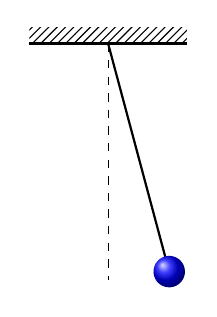
\begin{tikzpicture}
      \fill[pattern=north east lines] (-1,0) rectangle (1,.2);
      \draw[very thick] (-1,0)--(1,0);
      \begin{scope}[rotate=15]
        \draw[thick] (0,0)--(0,-3);% node[midway,right]{$\ell$};
        \shade[ball color=blue] (0,-3) circle (.2);
      \end{scope}
      \draw[dashed,thin] (0,0)--(0,-3);
    \end{tikzpicture}
    \begin{displaymath}
      K+U_g=\text{constant}
    \end{displaymath}
  \end{columns}  
\end{frame}


\begin{frame}{Oscillatory Systems}
  To understand how these systems oscillate, we have to go back to the
  dynamics (i.e.\ using free-body diagrams and second law of motion) of such
  a system.
  \begin{itemize}
  \item These types of oscillatory motion is called \textbf{harmonic motion}
  \item Solving these problems generally requires calculus
  \end{itemize}
\end{frame}


\section{Horizontal Spring-Mass}

%\begin{frame}{Quick Review of Hooke's Law}
%  \textbf{Hooke's law} relates the spring force $\vec F_e$ a
%  compressed/stretched spring exerts on objects connected to it to its
%  displacement $\vec x$:
%
%  \eq{-.1in}{
%    \boxed{\vec F_e=-k\vec x}
%  }
%  
%  where the \textbf{spring constant} $k$ is the stiffness of the spring. Spring
%  force is \emph{conservative}, and the elastic potential energy stored in the
%  spring is:
%
%  \eq{-.1in}{
%    \boxed{U_e=\frac12kx^2}
%  }
%\end{frame}



\begin{frame}{Horizontal Spring-Mass System}
  Assuming that there is no friction, drag or other damping forces, consider the
  forces acting on a mass connected horizontally to a spring:
  \begin{center}
    \vspace{-.1in}
    \begin{tikzpicture}[scale=.9]
      \draw[mass] (5,.5) rectangle +(1,1);
      \draw[thick,
        decoration={aspect=.3,segment length=2mm, amplitude=2.5mm, coil},
        decorate] (0,1)--(5,1);
      \fill[pattern=north east lines] (6.5,0.5)--(6.5,0.3)--(-0.2,0.3)
      --(-0.2,2)--(0,2)--(0,0.5)--cycle;
      \draw[very thick] (0,2)--(0,0.5)--(6.5,0.5);
      \draw[vectors,red] (5.5,1)--(5.5,0) node[right]{$m\vec g$};
      \draw[vectors,red] (5.5,1)--(5.5,2) node[right]{$\vec N$};
      \draw[vectors,red] (5.5,1)--(4.5,1) node[above]{$\vec F_e$};
      \fill[red] (5.5,1) circle (.07);
      \draw[axes] (7,1)--(7.8,1) node[right]{$+$};
      \draw[vectors] (3,1.65)--(5,1.65) node[midway,above]{$x$};
      \draw[dashed,thick] (3,0)--(3,2.3)
      node[above=-2]{\scriptsize equilibrium/unstretched position};
    \end{tikzpicture}
  \end{center}

  \vspace{-.15in}Net force is due only to spring force $F_e=-kx$. This is
  true both when the spring is in compression or extension.\footnote{In the
    diagram above, the spring is in extension.} Applying 2nd law of motion
  along the direction of motion:

  \eq{-.2in}{
    -kx=ma
  }

  \vspace{-.2in}This is a standard problem in calculus, with a well-known
  solution.
\end{frame}



\begin{frame}{A Simple Solution}
  The solution to this equation\footnote{Called a \emph{second-order ordinary
  differential equation with constant coefficient} in calculus} is
  simple\footnote{If you know calculus, that is. Otherwise it is quite
  impossible to solve}. There are two functions that can satisfy this equation: 
  $\cos$ and $\sin$. For a cosine, the position ($x$), velocity ($v$) and
  acceleration ($a$) of the mass as functions of time are given by:
 
  \vspace{-.3in}{\large
    \begin{align*}
      x(t)&=A\cos(\omega t)\\
      v(t)&=-A\omega\sin(\omega t)\\
      a(t)&=-A\omega^2\cos(\omega t)
    \end{align*}
    }

  where $\omega$ is the angular frequency of the oscillation, called the
  \textbf{natural frequency}, measured in \emph{radians per second}
  (\si{rad\per\second})\footnote{Angular frequency, or angular velocity,
  was introduced in Class 3, on circular motion}, and $A$ is the amplitude of
  the oscillation.
\end{frame}



\begin{frame}{A Simple Solution}
  Substituting the equations for position and acceleration into the original
  equation, we find that $\omega$ is related to mass and spring constant by:

  \eq{-.1in}{
    \boxed{\omega=\sqrt\frac km}
  }

  
  Frequency $f$ (number of oscillations per second, measured in \si{\hertz})
  and period $T$ (the time it takes for one oscillation, measured in
  \si\second) of the oscillation are:% related to $\omega$ by:

  \eq{-.1in}{
    \boxed{f=\frac{\omega}{2\pi}=\frac1{2\pi}\sqrt{\frac km}}
    \quad\text{\normalsize and}\quad
    \boxed{T=\frac1f=\frac{2\pi}{\omega}=2\pi\sqrt{\frac mk}}
  }

  Note that $f$ and $T$ do not depend on amplitude $A$.
\end{frame}


\begin{frame}{A Simple Oscillator}
  The sine/cosine solution to the differential equation is \emph{strictly}
  periodic, and the motion of such a system is called a
  \textbf{simple harmonic motion}.

  \vspace{-.3in}{\large
    \begin{align*}
      x(t)&=A\cos(\omega t)\\
      v(t)&=-A\omega\sin(\omega t)\\
      a(t)&=-A\omega^2\cos(\omega t)
    \end{align*}
    }

  In such a system, there are no external forces, and therefore the system is
  isolated.
\end{frame}



\begin{frame}{Motion Graphs}
  \begin{columns}
    \column{.48\textwidth}
    \begin{tikzpicture}[scale=.6]
      \draw[axes] (0,-1.5)--(0,2) node[right]{$x$};
      \draw[axes] (0,0)--(10,0) node[right]{$t$};
      \draw[thick] (-.2,1.2)--(0,1.2) node[left]{\scriptsize $A$};
      \draw[thick] (-.2,-1.2)--(0,-1.2) node[left]{\scriptsize $-A$};
    
      \draw[axes] (0,-5.5)--(0,-2) node[right]{$v$};
      \draw[axes] (0,-4)--(10,-4) node[right]{$t$};
      \draw[thick] (-.2,-2.8)--(0,-2.8) node[left]{\scriptsize $v_\text{max}$};
      \draw[thick] (-.2,-5.2)--(0,-5.2) node[left]{\scriptsize $-v_\text{max}$};
      
      \draw[axes] (0,-9.5)--(0,-6) node[right]{$a$};
      \draw[axes] (0,-8)--(10,-8) node[right]{$t$};
      \draw[thick] (-.2,-6.8)--(0,-6.8) node[left]{\scriptsize $a_\text{max}$};
      \draw[thick] (-.2,-9.2)--(0,-9.2) node[left]{\scriptsize $-a_\text{max}$};
      
      \begin{scope}[samples=80,smooth,domain=0:9,very thick]
        \draw[magenta] plot(\x,{1.2*cos(90*\x)});
        \draw[violet] plot(\x,{-1.2*sin(90*\x)-4});
        \draw[orange] plot(\x,{-1.2*cos(90*\x)-8});
      \end{scope}

      \uncover<2->{
        \fill[magenta] (4,1.2) circle (.1);
        \draw[thick,dotted,magenta] (4,1.2)--(4,-4);
        \fill[violet] (4,-4) circle (.1);

        \fill[magenta] (6,-1.2) circle (.1);
        \draw[thick,dotted,magenta] (6,-1.2)--(6,-4);
        \fill[violet] (6,-4) circle (.1);

        \fill[magenta] (8,1.2) circle (.1);
        \draw[thick,dotted,magenta] (8,1.2)--(8,-4);
        \fill[violet] (8,-4) circle (.1);
      }

      \uncover<3->{
        \draw[thick,dotted,magenta] (4,-4)--(4,-9.2);
        \fill[orange] (4,-9.2) circle (.1);

        \draw[thick,dotted,magenta] (6,-4)--(6,-6.8);
        \fill[orange] (6,-6.8) circle (.1);
        
        \draw[thick,dotted,magenta] (8,-4)--(8,-9.2);
        \fill[orange] (8,-9.2) circle (.1);
      }

      \uncover<4->{
        \draw[thick,dotted,violet] (1,0)--(1,-8);
        \fill[violet] (1,-5.2) circle (.1);
        \fill[magenta] (1,0) circle (.1);
        \fill[orange] (1,-8) circle (.1);

        \draw[thick,dotted,violet] (3,0)--(3,-8);
        \fill[violet] (3,-2.8) circle (.1);
        \fill[magenta] (3,0) circle (.1);
        \fill[orange] (3,-8) circle (.1);
        
        %\draw[thick,dotted,magenta] (6,-4)--(6,-6.8);
        %\fill[orange] (6,-6.8) circle (.1);
        %
        %\draw[thick,dotted,magenta] (8,-4)--(8,-9.2);
        %\fill[orange] (8,-9.2) circle (.1);
      }
    \end{tikzpicture}

    \column{.52\textwidth}
    \begin{itemize}
    \item<2->{\color{magenta}When the spring is fully extended or compressed
      ($x=\pm A$), $v=0$. At this time, the mass is \emph{momentarily} at rest}
    \item<3->{\color{magenta}At $x=\pm A$, $a=\mp a_\text{max}$, i.e.\
      acceleration is at maximum amplitude, but in the opposite direction. This
      is consistent with Hooke's law}
    \item<4->{\color{violet}Maximum speed $v_\text{max}$ occurs at the
      equilibrium position $x=0$, where acceleration is also zero $a=0$}
   \end{itemize}
  \end{columns}
\end{frame}



\begin{frame}{Cosine vs.\ Sine}
  When would the solution be a cosine, and when would it be a sine?

  \vspace{-.2in}\begin{columns}[T]
    \column{.47\textwidth}
    \begin{center}
      \begin{tikzpicture}[scale=.95]
        \draw[mass] (4,.5) rectangle +(1,1);
        \draw[thick,
          decoration={aspect=.3,segment length=2mm, amplitude=2.5mm, coil},
          decorate] (0,1)--(4,1);
        \fill[pattern=north east lines] (5.5,.5)--(5.5,.3)--(-.2,.3)
        --(-0.2,1.5)--(0,1.5)--(0,.5)--cycle;
        \draw[very thick] (0,1.5)--(0,.5)--(5.5,.5);
        \draw[vectors] (2.5,1.65)--(4,1.65) node[midway,above]{$x=+A$};
        \draw[dashed,thick] (2.5,.2)--(2.5,2)
        node[above=0]{\scriptsize equilibrium};
      \end{tikzpicture}
    \end{center}
    \vspace{-.1in}
    \textbf{Cosine:} The spring is initially stretched to $x=+A$, and the
    mass is released from rest at $t=0$.
    %If the spring is compressed to $x=-A$, use the $-\cos$ function.
    
    \column{.47\textwidth}
    \begin{center}
      \begin{tikzpicture}[scale=.95]
        \draw[mass] (2.5,.5) rectangle +(1,1);
        \draw[thick,
          decoration={aspect=.3,segment length=1.3mm, amplitude=2.5mm, coil},
          decorate] (0,1)--(2.5,1);
        \fill[pattern=north east lines] (5.5,.5)--(5.5,.3)--(-.2,.3)
        --(-0.2,1.5)--(0,1.5)--(0,.5)--cycle;
        \draw[very thick] (0,1.5)--(0,.5)--(5.5,.5);
        \draw[vectors] (3,1)--+(1,0) node[right]{$v=v_\text{max}$};
        \draw[dashed,thick] (2.5,.2)--+(0,1.8)
        node[above=0]{\scriptsize equilibrium};
      \end{tikzpicture}
    \end{center}
    \vspace{-.1in}
    \textbf{Sine:} If the mass is given a ``tap'' in the ($+$) direction at
    $t=0$ to give it an initial velocity of $v=v_\text{max}$.
    %If the mass is tapped in the ($-$) direction, use $-\sin$.
    \vspace{-.1in}
    \begin{align*}
      x(t)&=A\sin(\omega t)\\
      v(t)&=A\omega\cos(\omega t)\\
      a(t)&=-A\omega^2\sin(\omega t)
    \end{align*}
  \end{columns}
\end{frame}



\begin{frame}{Maximum Speed}
  The maximum speed (i.e.\ magnitude of velocity) of the mass is the
  ``amplitude'' of the velocity function:

  \eq{-.1in}{
    v(t) =-\underbracket[1pt]{A\omega}_{v_\text{max}}\sin(\omega t)
  }

  \vspace{-.05in}Substituting the expression for $\omega=\sqrt{k/m}$, we get
  
  \eq{-.1in}{
    v_\text{max}=A\omega=A\sqrt{\frac km}
  }

  We can also obtain this result by solving the law of conservation of energy
  problem. 
\end{frame}



\begin{frame}{Maximum Acceleration}
  Likewise, the maximum magnitude of acceleration of the mass is the
  ``amplitude'' of the acceleration function:

  \eq{-.1in}{
    a(t)=-\underbracket[1pt]{A\omega^2}_{a_\text{max}}\cos(\omega t)
  }

  \vspace{-.05in}Again, substituting the expression for $\omega=\sqrt{k/m}$, we
  get:
  
  \eq{-.1in}{
    a_\text{max}=A\omega^2=A\frac km
  }

  We can also obtain this result using the original differential equation.
\end{frame}



\section{Vertical Spring-Mass}

\begin{frame}{Vertical Spring-Mass System}
  \begin{columns}
    \column{.3\textwidth}
    \begin{tikzpicture}[scale=1.3]
      \draw[mass] (.7,1.7) rectangle(1.3,2.3);
      \draw[thick,
        decoration={aspect=0.3,segment length=2mm, amplitude=2.5mm, coil},
        decorate] (1,5)--(1,2.5); 
      \fill[pattern=north east lines] (0,5) rectangle (2,5.2);
      \draw[very thick] (0,5)--(2,5);
      \draw[vectors,red] (1,2)--(1,1.2) node[right]{$m\vec g$};
      \draw[vectors,red] (1,2)--(1,2.8) node[right]{$\vec F_e$};
      \fill[red] (1,2) circle (.05);
      \draw[axes] (1,1)--(1,.5) node[below]{$+$};
      \draw[vectors] (.3,4)--(.3,2.3) node[midway,left]{$x$};
      \draw[vectors] (1.7,4)--(1.7,3.5) node[midway,right]{$B$};
      \begin{scope}[thick,dashed]
        \draw (0,4)--(2,4) node[right]{\scriptsize unstretched};
        \draw (0,3.5)--(2,3.5) node[right]{\scriptsize equilibrium};
      \end{scope}
    \end{tikzpicture}
    
    \column{.7\textwidth}
    Assuming that there are no friction, drag and other damping forces, the
    analysis for a \textbf{vertical spring-mass system} is similar to the
    horizontal system, but with some important differences:
    \begin{itemize}
    %\item The isolated system includes the mass, spring and Earth
    \item The gravitational force ($m\vec g$) also acts along the direction of
      motion, and contributes to the net force
    \item $B$ is the stretching of the spring due to the weight:
    
      \eq{-.1in}{
        B=\frac{mg}k
      }
    \item The equilibrium position is \emph{not} the unstretched position
    \end{itemize}
%    \emph{slightly} more
%    complicated, but the result is very similar:
%
%    \vspace{-.35in}{\large
%      \begin{align*}
%        x(t) &= A\cos(2\pi ft)\textcolor{red}{ +B}\\
%        v(t) &= -2\pi Af\sin(2\pi ft)\\
%        a(t) &= -4\pi^2Af^2\cos(2\pi ft)
%      \end{align*}
%    }
%
%    \vspace{-.1in}Natural frequency $f$ and period $T$ are the same as the
%    horizontal spring-mass system
  \end{columns}
\end{frame}



\begin{frame}{Vertical Spring-Mass System}
  \begin{columns}
    \column{.3\textwidth}
    \begin{tikzpicture}[scale=1.3]
      \draw[mass] (.7,1.7) rectangle(1.3,2.3);
      \draw[thick,
        decoration={aspect=0.3,segment length=2mm, amplitude=2.5mm, coil},
        decorate] (1,5)--(1,2.5); 
      \fill[pattern=north east lines] (0,5) rectangle (2,5.2);
      \draw[very thick] (0,5)--(2,5);
      \draw[vectors,red] (1,2)--(1,1.2) node[right]{$m\vec g$};
      \draw[vectors,red] (1,2)--(1,2.8) node[right]{$\vec F_e$};
      \fill[red] (1,2) circle (.05);
      \draw[axes] (1,1)--(1,.5) node[below]{$+$};
      \draw[vectors] (.3,4)--(.3,2.3) node[midway,left]{$x$};
      \draw[vectors] (1.7,4)--(1.7,3.5) node[midway,right]{$B$};
      \begin{scope}[thick,dashed]
        \draw (0,4)--(2,4) node[right]{\scriptsize unstretched};
        \draw (0,3.5)--(2,3.5) node[right]{\scriptsize equilibrium};
      \end{scope}
    \end{tikzpicture}
    
    \column{.7\textwidth}
    The differential equation is \emph{slightly} more difficult than
    the horizontal system because of the gravitational force:

    \eq{-.2in}{
      mg-kx=ma
    }
    
    \vspace{-.2in}but the solution is similar, with the exception of the
    constant $\color{magenta}B$ in the position function $x(t)$:

    \vspace{-.32in}{\large
      \begin{align*}
        x(t) &= A\cos(\omega t)+{\color{magenta}B}\\
        v(t) &= -A\omega\sin(\omega t)\\
        a(t) &= -A\omega^2\cos(\omega t)
      \end{align*}
    }

    Angular frequency $\omega$, frequency $f$ and period $T$ of the oscillation
    are the same as the horizontal system
  \end{columns}
\end{frame}



%\section{Energy Conservation}
%
%\begin{frame}{Conservation of Energy in Spring-Mass Systems}
%  Since acceleration is non constant for spring-mass problems, we cannot use
%  kinematic equations to solve the motion problem. Instead, we can use
%  conservation of energy.
%  \begin{itemize}
%  \item Assuming that there is no friction or damping forces, the only forces
%    doing work are the spring force and gravitational force (for the vertical
%    system), both of which are conservative, therefore energy in the system is
%    conserved:
%
%    \eq{-.1in}{
%      K + U_e + U_g = K' + U_e' + U_g'
%    }
%    
%  \item\vspace{-.2in}For the horizontal spring-mass system, the total energy
%    can be evaluated at amplitude, when the mass is momentarily stationary,
%    and kinetic energy is zero:
%    
%    \eq{-.1in}{
%      E_\text{tot}=U_e + \cancel{K} = \frac12kA^2
%   }
%  \end{itemize}
%\end{frame}



\begin{frame}{Simple Example}
  \textbf{Example:} A mass suspended from a spring is oscillating up and
  down. Consider the following two statements:
  \begin{enumerate}
  \item At some point during the oscillation, the mass has zero velocity but it
    is accelerating
  \item At some point during the oscillation, the mass has non-zero velocity and
    zero acceleration.
  \end{enumerate}
  \begin{enumerate}[(A)]
  \item Both occur at some time during the oscillation
  \item Neither occurs during the oscillation
  \item Only (1) occurs
  \item Only (2) occurs
  \end{enumerate}
\end{frame}



\begin{frame}{Another Example}
  \textbf{Example:} An object of mass \SI{5.0}{\kilo\gram} hangs from a spring
  and oscillates with a period of \SI{0.50}\second. By how much will the
  equilibrium length of the spring be shortened when the object is removed.
  \begin{enumerate}[(A)]
  \item\SI{.75}{\centi\metre}
  \item\SI{1.5}{\centi\metre}
  \item\SI{3.1}{\centi\metre}
  \item\SI{6.2}{\centi\metre}
  \end{enumerate}
\end{frame}



\section{Simple Pendulum}

\begin{frame}{What About a Simple Pendulum?}
  \begin{columns}
    \column{.75\textwidth}
    Simple pendulums also exhibit simple harmonic motion
    \begin{itemize}
    \item Two forces act on the mass: gravity $F_g=mg$ and tension $F_T$
    \item When the pendulum is deflected by an angle $\theta$, there is a
      component of gravity pointing towards the rest position, with magnitude
      $mg\sin\theta$
    \item For small angles, $\sin\theta\approx\theta$, so this force is
      approximately proportional $\theta$ (very similar to Hooke's law where
      $F_e\propto x$)
    \end{itemize}

    \column{.25\textwidth}
    \begin{tikzpicture}
      \fill[pattern=north east lines] (-1,0) rectangle (1,0.2);
      \draw[very thick] (-1,0)--(1,0);
      \begin{scope}[rotate=20]
        \draw[thick] (0,0)--(0,-5) node[midway,right]{$\ell$};
        \shade[ball color=red] (0,-5) circle (.2) node[below right]{$m$};
        \draw[dotted,vectors,red] (0,-5)--+(-.75,0)
        node[left,fill=yellow!15]{$mg\sin\theta$};
        \draw[vectors,red] (0,-5)--(0,-3) node[left]{$\vec F_T$};
        \draw[vectors,red,rotate around={-20:(0,-5)}] (0,-5)--+(0,-1.5)
        node[below]{$m\vec g$};
      \end{scope}
      \draw[dashed,thin] (0,0)--(0,-5);
      \draw[axes] (0,-2) arc (270:290:2) node[midway,below]{$\theta$};
    \end{tikzpicture}
  \end{columns}
\end{frame}



\begin{frame}{Equation for the Pendulum}
  When $\theta$ is small, the restoring force acts like a spring, and
  the solution for $\theta(t)$ has the same form as the spring-mass system:

  \eq{-.1in}{
    \boxed{\theta(t)=\theta_\text{max}\cos(\omega t)}
  }

  where maximum angle $\theta_\text{max}$ is the amplitude of the oscillation,
  and natural (angular) frequency $\omega$, frequency $f$, and period $T$
  are given by
    
  \eq{-.13in}{
    \boxed{\omega=\sqrt\frac g\ell}
    \quad\quad
    \boxed{f=\frac{\omega}{2\pi}=\frac1{2\pi}\sqrt{\frac g\ell}}
    \quad\quad
    \boxed{T=\frac1f=2\pi\sqrt{\frac\ell{g}}}
  }

  Like the spring-mass systems, $\omega$, $f$ and $T$ of the pendulum
  system do not depend on amplitude, but \emph{unlike} the spring-mass
  systems, they also do not depend on mass $m$.
\end{frame}



\begin{frame}{How Good is the Small-Angle Approximation?}
  \begin{center}
    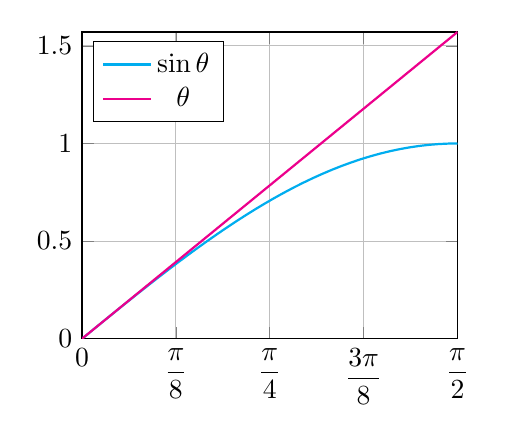
\begin{tikzpicture}
      \begin{axis}[
          width=2.5in,
          xmin=0,xmax=pi/2,
          ymin=0,ymax=pi/2,
          %xlabel=$\theta$ (radian),
          xtick={0,pi/8,pi/4,3*pi/8,pi/2},
          xticklabels={
            0,$\dfrac\pi8$,$\dfrac\pi4$,$\dfrac{3\pi}8$,$\dfrac\pi2$
          },
          grid = both,
          legend pos=north west,
        ]
        \addplot[
          color=cyan,
          domain=0:pi/2,
          samples=40,
          style={thick}]{sin(x*180/pi)};
        \addlegendentry{$\sin\theta$}
        \addplot[
          color=magenta,
          domain=0:pi/2,
          samples=40,
          thick]{x};
        \addlegendentry{$\theta$}
      \end{axis}
    \end{tikzpicture}
    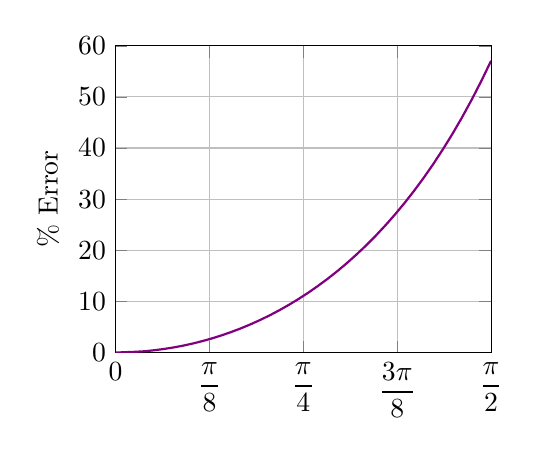
\begin{tikzpicture}
      \begin{axis}[
          width=2.5in,
          ylabel=\% Error,
          xmin=0,xmax=pi/2,
          ymin=0,ymax=60,
          %xlabel=$\theta$ (radian),
          xtick={0,pi/8,pi/4,3*pi/8,pi/2},
          xticklabels={
            0,$\dfrac\pi8$,$\dfrac\pi4$,$\dfrac{3\pi}8$,$\dfrac\pi2$
          },
          ytick={0,10,...,60},
          legend pos=north west,
          grid = both,
        ]
        \addplot[
          color=violet,
          domain=0:pi/2,
          samples=40,
          style=thick
        ]{abs(sin(x*180/pi)-x)/sin(x*180/pi)*100};
      \end{axis}
    \end{tikzpicture}
  \end{center}
  What the maximum angle of deflection can be used depends on the precision
  that the answer requires.
\end{frame}



\begin{frame}{Example Problem}
  \textbf{Example:} A simple pendulum consists of a mass $m$ attached to a
  light string of length $\ell$. If the system is oscillating through small
  angles, which of the following is true?
  \begin{enumerate}[(A)]
  \item The frequency is independent of the acceleration due to gravity $g$.
  \item The period depends on the amplitude of the oscillation.
  \item The period is independent of the mass $m$.
  \item The period is independent of the length $\ell$.
  \end{enumerate}
\end{frame}



\begin{frame}{Example Problem}
  \textbf{Example:} A bucket full of water is attached to a rope and allowed
  to swing back and forth as a pendulum from a fixed support. The bucket has a
  hole in its bottom that allows water to leak out. How does the period of
  oscillatory motion change with the loss of water?
  \begin{enumerate}[(A)]
  \item The period does not change.
  \item The period continuously decreases.
  \item The period continuously increases.
  \item The period increases to some maximum and then decreases again.
  \end{enumerate}
\end{frame}



\begin{frame}{Think About $g$}
  \textbf{Example:} A young girl is playing with a toy pendulum while riding
  in an elevator. Being an astute observer, she notes that the period of the
  pendulum is \SI{2.0}\second. Suddenly the cables supporting the elevator
  break, and all of the brakes and safety features fail simultaneously. The
  elevator plunges into free fall. The girl is astonished to discover that the
  pendulum \underline{\hspace{1in}}
  \begin{enumerate}[(A)]
  \item continues oscillating with a period of \SI{2.0}\second.
  \item stops oscillating entirely.
  \item decreases its rate of oscillation to have a longer period.
  \item increases its rate of oscillation to have a lesser period.
  \end{enumerate}
\end{frame}



\section{Damped Oscillators}

\begin{frame}{It's Never Perfect}
  In reality, oscillatory systems have kinetic friction, drag, and other
  damping forces that take away energy. For a horizontal spring-mass systems,
  we can represent these forces by a shock absorber along the direction of
  motion:
  \begin{center}
    \begin{tikzpicture}
      \draw[lightgray,thick,fill=cyan!10] (3,.5) rectangle (4,1.5);
      \draw[thick,lightgray,decorate,
        decoration={aspect=.4,segment length=5.5,amplitude=6,coil}]
      (0,1)--(3,1);
      \fill[thick,draw=lightgray,pattern=north east lines] (-.2,2)--(-.2,.3)
      --(6.7,.3)--(6.7,2) --(6.5,2) --(6.5,.5)--(0,.5)--(0,2)--cycle;
      \draw[axes] (7,1)--+(1,0) node[right]{$+$};

      %shock absorber
      \draw[fill=pink!70] (4.9,.8) rectangle (5.5,1.2);
      \begin{scope}[very thick]
        \draw (4.05,1)--(4.9,1);
        \draw (4.9,.8)--(4.9,1.2);
        \draw (4.8,1.2)--(5.5,1.2)--(5.5,.8)--(4.8,.8);
        \draw (5.5,1)--(6.5,1);
      \end{scope}
      
      \draw[vectors,red] (3.5,1)--+(0,-1) node[below]{$m\vec g$};
      \draw[vectors,red] (3.5,1)--+(0,1) node[above]{$\vec N$};
      \draw[vectors,red] (3.5,1)--+(-1,0) node[above]{$\vec F_e$};
      \draw[vectors,violet] (3.5,1)--+(1,0) node[below]{$\vec F_D$};
      \fill[red] (3.5,1) circle (.075);
    \end{tikzpicture}
  \end{center}
  The combined friction, drag, and damping forces are grouped into a single
  force ``$\vec F_D$''.
\end{frame}



\begin{frame}{Damped Oscillators}
  In general, the damping force is a function of velocity, and acts in the
  opposite direction to the motion of the mass:
  
  \eq{-.22in}{
    F_D=-bv^n
  }

  \vspace{-.15in}The positive constant $b$ is called the \textbf{damping
    factor}.
  \begin{itemize}
  \item For kinetic friction, $n=0$
  \item For aerodynamic drag, $n=2$, and
  \item For viscous damping, $n\approx 1$
  \end{itemize}
  Usually there is a combination of these forces, so we use $n=1$ to
  approximate the \emph{average}\footnote{Whether this is
  \emph{accurate} will depend on the specific problem that needs to be solved.}.
  Applying the 2nd law of motion, the differential equation is more complicated:
  
  \eq{-.2in}{
    -kx-bv=ma
  }
\end{frame}



\begin{frame}{Damped Oscillators}
  The solution this equation is still a standard\footnote{Albeit a
  substantially more difficult problem in calculus} calculus problem. The
  motion of the mass now also has a {\color{magenta}exponential decay} term:

  \eq{-.1in}{
    x(t)=
    \underbracket[1pt]{\color{magenta}A_0e^{-\frac b{2m}t}}_\text{amplitude}
    \cos(\omega't)
  }

  where $A_0$ is the initial amplitude when oscillation begins,
  and frequency $\omega'$ now decreases from the natural frequency, i.e.:

  \eq{-.1in}{
    \omega'<\omega
  }
  %As damping factor $b$ increases, it becomes
  %critical $b_c$, and the system no longer oscillates.

%  \eq{-.1in}{
%    \omega'=\sqrt{\omega^2-\left(\frac b{2m}\right)^2}
%    \quad{\text{\normalsize where}}\quad
%    \omega=\sqrt{\frac km}
%  }

%  Angular frequency $\omega'$ of the damped oscillator decreases from the
%  undamped case $\omega$ depending on the damping factor $b$. (Lower frequency,
%  longer period.)
\end{frame}



\begin{frame}{Critical Damping}
  As the damping factor $b$ increases, the angular frequency $\omega'$
  decreases, leading to a longer period $T$:
  
  \eq{-.15in}{
    \omega'=\sqrt{\omega^2-\left(\frac b{2m}\right)^2}
  }

  \textbf{Critical damping} occurs when the angular frequency $\omega'=0$,
  and the system no longer oscillates. This occurs at
  \textbf{critical damping factor} of:

  \eq{-.1in}{
    b_c=2m\omega=2\sqrt{km}
  }
  \begin{itemize}
  \item\vspace{-.1in}A critically damped system returns to its equilibrium
    position in the shortest time with \emph{no} oscillation
  \item When $b>b_c$, the system is \textbf{over-damped}
  \item Critical or near-critical damping is desired in many engineering designs
    (e.g.\ shock absorbers on car suspensions)
  \end{itemize}
\end{frame}



\begin{frame}{Damped Oscillators}
  \begin{columns}[T]
    \column{.25\textwidth}
    \begin{center}
      \vspace{-.2in}
      \begin{tikzpicture}
        \draw[axes] (0,0)--(3,0) node[right]{$t$};
        \draw[axes] (0,-1.2)--(0,1.5) node[right]{$x$};
        \draw[samples=100,domain=0:2.7,functions] plot(\x,{1.2*(cos(500*\x)});
      \end{tikzpicture}
    \end{center}
    
    {\footnotesize In an \textbf{undamped} oscillator ($b=0$), the motion of
      the mass or pendulum is strictly periodic.\par}
    
    \column{.25\textwidth}
    \begin{center}
      \vspace{-.2in}
      \begin{tikzpicture}
        \draw[axes] (0,0)--(3,0) node[right]{$t$};
        \draw[axes] (0,-1.2)--(0,1.5) node[right]{$x$};
        \draw[samples=100,domain=0:2.7,functions]
        plot(\x,{1.2*exp(-.7*\x)*(cos(400*\x)});
        \draw[samples=10,domain=0:2.7,thick,dashed] plot(\x,{1.2*exp(-.7*\x)});
      \end{tikzpicture}
    \end{center}

    {\footnotesize Amplitude of an \textbf{under-damped} oscillator ($b<b_c$)
      decays with time. The motion is \emph{quasi} periodic. Frequency $f'$
      decreases with increasing damping factor $b$.\par}

    \column{.25\textwidth}
    \begin{center}
      \vspace{-.2in}
      \begin{tikzpicture}
        \draw[axes] (0,0)--(3,0) node[right]{$t$};
        \draw[axes] (0,-1.2)--(0,1.5) node[right]{$x$};
        \draw[samples=20,domain=0:2.7,functions] plot(\x,{1.2*exp(-1.5*\x)});
      \end{tikzpicture}
    \end{center}

    {\footnotesize In a \textbf{critically damped} system ($b=b_c$), the mass
      or pendulum no longer oscillates. The motion only decays
      exponentially.\par}
    
    \column{.25\textwidth}
    \begin{center}
      \vspace{-.2in}
      \begin{tikzpicture}
        \draw[axes] (0,0)--(3,0) node[right]{$t$};
        \draw[axes] (0,-1.2)--(0,1.5) node[right]{$x$};
        \draw[samples=20,domain=0:2.7,functions] plot(\x,{1.2*exp(-.5*\x)});
      \end{tikzpicture}
    \end{center}
    
    {\footnotesize The motion of an \textbf{over-damped} system ($b>b_c$) is
      still an exponential decay, but the decay rate is slow because of the
      damping force.\par}
  \end{columns}
\end{frame}


\section{Driven Oscillators}

\begin{frame}{Driven Oscillators}
  To keep a damped system going, energy must be added into the system.
  \begin{center}
    \begin{tikzpicture}
      \draw[thick,lightgray,fill=cyan!10] (3,.5) rectangle (4,1.5);
      \draw[thick,lightgray,
        decoration={aspect=.35,segment length=2.5mm, amplitude=2.5mm, coil},
        decorate] (0,1)--(2.95,1);
      \fill[pattern=north east lines] (-.5,2)--(-.5,0)--(7,0)--(7,2)--(6.5,2)
      --(6.5,.5)--(0,.5)--(0,2)--cycle;
      \draw[thick,gray] (0,2)--(0,.5)--(6.5,.5)--(6.5,2);
      \draw[fill=pink!60] (4.9,.8) rectangle (5.5,1.2);
      \begin{scope}[very thick,gray]
        \draw(4.05,1)--(4.9,1);
        \draw(4.9,.8)--(4.9,1.2);
        \draw(4.8,1.2)--(5.5,1.2)--(5.5,.8)--(4.8,.8);
        \draw(5.5,1)--(6.5,1);
      \end{scope}
      \fill[red!60] (3.5,1) circle (.075);
      \begin{scope}[vectors,red]
        \draw (3.5,1)--(3.5,0) node[below]{$m\vec g$};
        \draw (3.5,1)--(3.5,2) node[above]{$\vec N$};
        \draw (3.5,1)--(2.5,1) node[above]{$\vec F_e$};
        \draw (3.5,1)--(4.5,1) node[below]{$\vec F_D$};
      \end{scope}
      \draw[vectors,violet] (3.5,.95)--(2,.95)
      node[left,fill=yellow!30,opacity=.8]{$\vec F_\text{ext}$};
    \end{tikzpicture}
  \end{center}
  Assume that the system is subjected to an external force
  $\vec F_\text{ext}(t)$ that is sinusoidal with time, with a
  \textbf{driving frequency} $\omega_e$:

  \eq{-.2in}{
    F_\text{ext}(t)=F_0\cos(\omega_e t)
  }  
\end{frame}



\begin{frame}{Forced Harmonic Motion}
  Accounting for all the horizontal forces, and applying the 2nd law of motion:
  
  \eq{-.1in}{
    -kx-bv+F_0\cos(\omega_et)=ma
  }

  \vspace{-.1in}This is a difficult problem even for calculus students, but
  it still has a well-studied solution:
  
  \eq{-.1in}{
    \boxed{x(t)=A\cos(\omega_et-\phi)}
  }
  
  The equation is in the same form as the SHM case, but the amplitude $A$ and
  phase shift $\phi$ are now given by:
  
  \eq{-.1in}{
    A=\frac{F_0}{\sqrt{m^2(\omega^2-\omega_e^2)^2+b^2\omega_e^2}}
    \quad\;\;
    \phi=\tan^{-1}\left[\frac{b\omega_e}{m(\omega^2-\omega_e^2)}\right]
  }
\end{frame}



\begin{frame}{Resonance}
  \textbf{Resonance} is caused by in-phase excitation at natural frequency.
  This means that:
  \begin{itemize}
  \item The frequency of the driving force near the natural frequency of
    the undamped oscillator

    \eq{-.1in}{
      \omega_e\approx\omega=\sqrt{\frac km}
    }
  \item The driving force follows the motion of the oscillator.
  \end{itemize}
\end{frame}



\begin{frame}{Resonance}
  Looking at the expression for amplitude of the oscillation with small value
  of $b$:
  
  \eq{-.1in}{
    A=\frac{F_0}{\sqrt{m^2(\omega^2-\omega_e^2)^2+b^2\omega_e^2}}
  }
  
  Amplitude is at maximum when the frequency of the driving force
  $\omega_e\approx\omega$, with a maximum value of:
  
  \eq{-.1in}{
    A_\text{max}\approx\frac{F_0}{b\omega_e}
  }
\end{frame}



\begin{frame}{Resonance}
  \begin{columns}
    \column{.45\textwidth}
    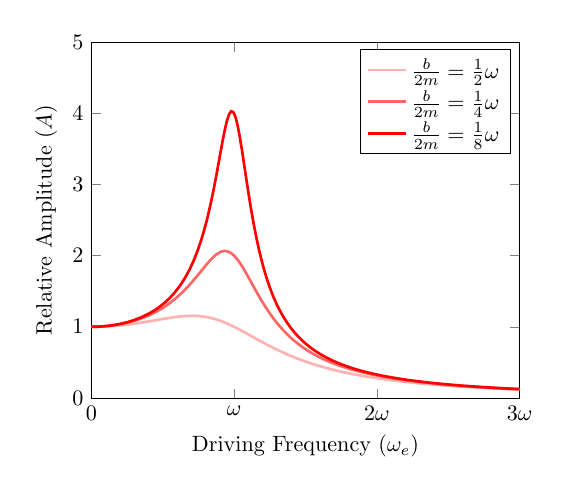
\begin{tikzpicture}[scale=.8]
      \begin{axis}[
          width=3.3in,
          xmin=0,xmax=3, xlabel=Driving Frequency ($\omega_e$),
          xtick={0,1,2,3}, xticklabels={0,$\omega$,$2\omega$,$3\omega$},
          ymin=0,ymax=5, ylabel=Relative Amplitude ($A$),
        ]
        \addplot[
          color=red!30,
          samples=300,
          domain=0:3,
          very thick]{1/sqrt((1-x^2)^2+x^2)};
        \addlegendentry{$\frac b{2m}=\frac12\omega$}
        \addplot[
          color=red!60,
          samples=200,
          domain=0:3,
          very thick]{1/sqrt((1-x^2)^2+x^2/4)};
        \addlegendentry{$\frac b{2m}=\frac14\omega$}
        \addplot[
          color=red,
          samples=200,
          domain=0:3,
          very thick]{1/sqrt((1-x^2)^2+x^2/16)};
        \addlegendentry{$\frac b{2m}=\frac18\omega$}
      \end{axis}
    \end{tikzpicture}
    
    \column{.55\textwidth}
    Plotting amplitude $A$ as a function of driving frequency $\omega_e$ shows
    that:
    \begin{itemize}
    \item For a lightly-damped system, resonance response is highest when
      $\omega_e\approx\omega$
    \item The smaller the damping constant $b$, the higher and narrower the
      peak is
    \end{itemize}
  \end{columns}
\end{frame}



\begin{frame}{Resonance}

  \eq{-.01in}{
    \boxed{\tan\phi=\frac{b\omega_e}{m(\omega^2-\omega_e^2)}}
  }

  When $\omega_e=\omega$ is substituted into the phase shift expression, the
  right-hand side becomes undefined. From this, we obtain a phase shift of
  $\varphi=\pi/2$. Using the expression for $v(t)$, and substituting
  $\varphi=\pi/2$:
  
  \eq{-.1in}{
    v(t)=-A\omega_e\sin\left(\omega_e t-\frac{\pi}2\right)
    =A\omega\cos(\omega_e t)
  }
\end{frame}



\begin{frame}{Resonance}
  At resonance, the object is always moving in the same direction as the
  driving force:

  \vspace{-.2in}{\large
    \begin{align*}
      v(t)&=A\omega\cos(\omega_e t)\\
      F_\text{ext}(t)&=F_0\cos(\omega_e t)
    \end{align*}
  }
\end{frame}
\end{document}
